% =============================================================================
%  TRABAJO PRÁCTICO INTEGRADOR · PRIMERA PARTE
%  Arquitectura de un e-commerce por capas
%
%  Compilar con:  xelatex TP_Primera_Parte_Ecommerce.tex   (dos pasadas)
%  Requiere las tipografías Inter, Inter Display y JetBrains Mono.
% =============================================================================
\documentclass[11pt,a4paper]{article}

\usepackage[a4paper,left=1.8cm,right=1.8cm,top=2.35cm,bottom=1.9cm,
            headheight=15pt,headsep=8mm,footskip=11mm]{geometry}
\usepackage{fontspec}
\usepackage[table]{xcolor}
\usepackage{tikz}
\usetikzlibrary{arrows.meta,positioning,fit,backgrounds,calc,shapes.geometric}
\usepackage[most]{tcolorbox}
\usepackage{tabularx}
\usepackage{booktabs}
\usepackage{array}
\usepackage{enumitem}
\usepackage{fancyhdr}
\usepackage{microtype}
\usepackage[hidelinks]{hyperref}

% ------------------------------------------------------------------ TIPOGRAFÍA
\setmainfont{Inter}[
  Path       = /usr/share/fonts/opentype/inter/,
  Extension  = .otf,
  UprightFont     = Inter-Regular,
  ItalicFont      = Inter-Italic,
  BoldFont        = Inter-SemiBold,
  BoldItalicFont  = Inter-SemiBoldItalic,
  Numbers    = Lining
]
\newfontfamily\displayfont{InterDisplay}[
  Path       = /usr/share/fonts/opentype/inter/,
  Extension  = .otf,
  UprightFont     = InterDisplay-Regular,
  ItalicFont      = InterDisplay-Italic,
  BoldFont        = InterDisplay-Bold,
  BoldItalicFont  = InterDisplay-BoldItalic
]
\newfontfamily\lightfont{Inter}[
  Path = /usr/share/fonts/opentype/inter/, Extension = .otf,
  UprightFont = Inter-Light, BoldFont = Inter-Medium
]
\setmonofont{JetBrainsMono}[
  Path       = /usr/share/fonts/truetype/jetbrains-mono/,
  Extension  = .ttf,
  UprightFont     = JetBrainsMono-Regular,
  ItalicFont      = JetBrainsMono-Italic,
  BoldFont        = JetBrainsMono-Bold,
  Scale      = 0.86
]
\newcommand{\track}[2]{{\addfontfeature{LetterSpace=#1}#2}}

% ---------------------------------------------------------------------- COLORES
\definecolor{navy}{HTML}{16243F}
\definecolor{steel}{HTML}{2C4A73}
\definecolor{brand}{HTML}{2A7BA8}
\definecolor{sky}{HTML}{6FB9D6}
\definecolor{pale}{HTML}{EAF4FA}
\definecolor{amber}{HTML}{E9A02B}
\definecolor{amberdk}{HTML}{A96F16}
\definecolor{ink}{HTML}{1E2A3C}
\definecolor{muted}{HTML}{6B7C93}
\definecolor{rule}{HTML}{D9E2EC}
\definecolor{surface}{HTML}{F4F7FA}
\definecolor{ok}{HTML}{2E7D5B}
\definecolor{no}{HTML}{AF4A40}

\hypersetup{colorlinks=true,linkcolor=brand,urlcolor=brand}

% Glifos dibujados: independientes de las fuentes matemáticas
\newcommand{\arr}{\,\tikz[baseline=-0.52ex,x=1ex,y=1ex]{%
  \draw[-{Latex[length=1.05ex,width=0.85ex]},line width=0.17ex,draw=amber]
        (0,0) -- (2.0,0);}\,}
\newcommand{\arrs}{\,\tikz[baseline=-0.52ex,x=1ex,y=1ex]{%
  \draw[-{Latex[length=0.95ex,width=0.75ex]},line width=0.15ex,draw=steel]
        (0,0) -- (1.7,0);}\,}
\newcommand{\tick}{\tikz[baseline=-0.35ex,x=1ex,y=1ex]{%
  \draw[ok,line width=0.24ex,line cap=round,line join=round]
        (0,0.55) -- (0.62,-0.12) -- (1.8,1.3);}}

% ---------------------------------------------------------------------- AJUSTES
\setlength{\parindent}{0pt}
\setlength{\parskip}{5pt}
\setlist[itemize]{leftmargin=4.5mm,itemsep=2.5pt,topsep=3pt,
                  label=\textcolor{sky}{\rule[1pt]{3pt}{3pt}}}
\setlist[enumerate]{leftmargin=6.5mm,itemsep=2.5pt,topsep=3pt,font=\bfseries\color{brand}}
\color{ink}
\arrayrulecolor{rule}
\setlength{\tabcolsep}{5pt}
\renewcommand{\arraystretch}{1.15}
\renewcommand\tabularxcolumn[1]{m{#1}}
\newcolumntype{L}[1]{>{\raggedright\arraybackslash}m{#1}}
\newcolumntype{M}[1]{>{\raggedright\arraybackslash\ttfamily\color{steel}}m{#1}}
\newcolumntype{N}[1]{>{\raggedright\arraybackslash\bfseries\color{navy}}m{#1}}
\newcommand{\thd}[1]{\normalfont\footnotesize\bfseries\color{muted}\track{6}{#1}}

\pagestyle{fancy}
\fancyhf{}
\lhead{\footnotesize\color{muted}\track{6}{DESARROLLO DE APLICACIONES II}%
       \ \ \textcolor{sky}{|}\ \ TP Integrador · Primera parte}
\rhead{\footnotesize\color{muted}TPO Store}
\cfoot{\footnotesize\color{muted}\thepage}
\renewcommand{\headrulewidth}{0.5pt}
\renewcommand{\headrule}{\hbox to\headwidth{\color{rule}\leaders\hrule height \headrulewidth\hfill}}

% -------------------------------------------------------------- TÍTULOS Y CAJAS
\newcommand{\sectiontitle}[2]{%
  \vspace{0.5mm}
  {\footnotesize\bfseries\color{amberdk}\track{9}{#1}}\par\vspace{1.4mm}
  {\displayfont\fontsize{20}{23}\selectfont\bfseries\color{navy}#2}\par
  \vspace{2.2mm}\textcolor{rule}{\rule{\linewidth}{0.8pt}}\vspace{0.5mm}
}
\newcommand{\blocktitle}[1]{%
  \vspace{1.2mm}{\displayfont\normalsize\bfseries\color{navy}#1}\par\vspace{-1.5mm}
}

\newtcolorbox{callout}[1][]{
  enhanced, colback=navy, colframe=navy, coltext=white, boxrule=0pt,
  arc=2.2mm, left=5mm, right=5mm, top=3.4mm, bottom=3.4mm,
  borderline west={2.4pt}{0pt}{amber}, #1}
\newtcolorbox{softbox}[1][]{
  enhanced, colback=pale, colframe=sky!55, boxrule=0.6pt, arc=2.2mm,
  left=4mm, right=4mm, top=3mm, bottom=3mm, #1}
\newtcolorbox{whitebox}[1][]{
  enhanced, colback=white, colframe=rule, boxrule=0.6pt, arc=2.2mm,
  left=4mm, right=4mm, top=3mm, bottom=3mm, #1}
\newtcolorbox{listbox}[2][]{
  enhanced, colback=white, colframe=#2, boxrule=0.7pt, arc=2.2mm,
  left=4mm, right=4mm, top=2.4mm, bottom=2.8mm,
  title=#1, fonttitle=\footnotesize\bfseries, coltitle=white, colbacktitle=#2,
  attach boxed title to top left={xshift=3mm,yshift=-2.2mm},
  boxed title style={boxrule=0pt,arc=1.2mm,left=2.5mm,right=2.5mm,top=0.8mm,bottom=0.8mm}}

% Estilos compartidos de diagramas
\tikzset{
  cbox/.style   = {draw=rule, line width=0.6pt, fill=white, rounded corners=2.2pt,
                   align=center, font=\small\bfseries, text=navy},
  chip/.style   = {draw=none, fill=surface, rounded corners=1.6pt, inner xsep=3.6pt,
                   inner ysep=2.6pt, font=\scriptsize\ttfamily, text=steel,
                   anchor=north west},
  call/.style   = {-{Latex[length=2.1mm,width=1.7mm]}, line width=0.75pt, draw=steel},
  evt/.style    = {-{Latex[length=2.1mm,width=1.7mm]}, line width=0.75pt, draw=amberdk,
                   dash pattern=on 2.2pt off 1.8pt},
  lbl/.style    = {font=\scriptsize, text=muted, inner sep=1.4pt},
}

\begin{document}

% =============================================================================
% PORTADA
% =============================================================================
\thispagestyle{empty}
\begin{tikzpicture}[remember picture,overlay]
  \fill[navy] (current page.north west) rectangle ([yshift=-12.6cm]current page.north east);
  % motivo: pila de tres capas
  \begin{scope}[shift={([xshift=-2.5cm,yshift=-6.6cm]current page.north east)}]
    \foreach \i/\o in {0/0.10, 1/0.17, 2/0.26}{
      \fill[white,opacity=\o,rounded corners=2pt]
        (-1.7+0.34*\i, -0.72*\i) rectangle ++(3.4,0.46);
    }
    \draw[amber,line width=1pt,-{Latex[length=1.8mm]}] (1.2,-0.05) -- (1.2,-1.42);
  \end{scope}
  % filetes de marca
  \fill[amber]  ([xshift=1.8cm,yshift=-1.7cm]current page.north west) rectangle ++(1.35cm,0.12cm);
  \fill[sky]    ([xshift=3.35cm,yshift=-1.7cm]current page.north west) rectangle ++(0.4cm,0.12cm);
\end{tikzpicture}

\vspace*{1.75cm}
{\footnotesize\bfseries\color{amber}\track{14}{TRABAJO PRÁCTICO INTEGRADOR · PRIMERA PARTE}}\par
\vspace{9mm}
{\displayfont\fontsize{35}{40}\selectfont\bfseries\color{white}
Arquitectura de un\\e-commerce por capas}\par
\vspace{7mm}
{\lightfont\Large\color{sky}Componentes, contratos, tecnologías\\y recorrido de un caso de uso real}\par

\vspace{4.7cm}

{\displayfont\bfseries\color{navy}\large TPO Store}\par
\vspace{-2.5mm}
{\color{muted}\small Plataforma de comercio electrónico · documento de arquitectura inicial}\par
\vspace{3mm}
\textcolor{rule}{\rule{\linewidth}{0.8pt}}
\vspace{1mm}

{\small
\begin{tabularx}{\linewidth}{@{}>{\footnotesize\bfseries\color{muted}}m{2.55cm}X
                              @{\hspace{7mm}}>{\footnotesize\bfseries\color{muted}}m{2.75cm}X@{}}
MATERIA   & Desarrollo de Aplicaciones II                   & ENTORNO      & Visual Studio Code · JDK 17+ \\
DOCUMENTO & Arquitectura y mockup técnico                   & CONSTRUCCIÓN & Apache Maven · WAR \\
GRUPO     & \textit{\color{muted}[completar integrantes]}   & PLATAFORMA   & Jakarta EE sobre WildFly \\
\end{tabularx}}

\vspace{7mm}
{\footnotesize\bfseries\color{muted}\track{9}{CONTENIDO DEL DOCUMENTO}}\par
\vspace{2mm}
{\small
\begin{tabularx}{\linewidth}{@{}>{\bfseries\color{amber}}m{7mm}X @{\hspace{7mm}}>{\bfseries\color{amber}}m{7mm}X@{}}
01 & Visión del proyecto                     & 04 & Recorrido entre capas \\
02 & Programación orientada a componentes    & 05 & Diseño y calidad \\
03 & Arquitectura de capas                   & 06 & Tecnología y entregable \\
\end{tabularx}}

\vfill
\begin{callout}
\textbf{Propósito académico.} Diseñar una aplicación orientada a componentes donde presentación, negocio y datos permanezcan claramente separados, con contratos explícitos, patrones justificados y un recorrido funcional de punta a punta.
\end{callout}

\newpage

% =============================================================================
% 01 · VISIÓN
% =============================================================================
\sectiontitle{01 · VISIÓN DEL PROYECTO}{Qué problema resuelve el e-commerce}

TPO Store permite que un cliente consulte un catálogo, administre su carrito y confirme una compra. Un administrador mantiene productos y stock. El alcance busca demostrar los contenidos de la materia sin incorporar complejidad comercial innecesaria.

\begin{callout}
\textbf{Idea rectora:} el valor del TP no está solamente en que ``la tienda funcione'', sino en poder explicar cómo cada petición atraviesa componentes y capas sin mezclar responsabilidades.
\end{callout}

\vspace{2mm}
\begin{minipage}[t]{0.485\linewidth}
\begin{listbox}[Cliente]{brand}
\begin{itemize}
  \item Registrarse e iniciar sesión.
  \item Explorar y buscar productos.
  \item Agregar, modificar o quitar ítems.
  \item Confirmar una compra.
  \item Consultar pedidos realizados.
\end{itemize}
\end{listbox}
\end{minipage}\hfill
\begin{minipage}[t]{0.485\linewidth}
\begin{listbox}[Administrador]{steel}
\begin{itemize}
  \item Crear y editar productos.
  \item Activar o desactivar publicaciones.
  \item Actualizar existencias.
  \item Consultar pedidos y estados.
  \item Revisar operaciones rechazadas.
\end{itemize}
\end{listbox}
\end{minipage}

\vspace{3mm}
\blocktitle{Alcance funcional mínimo}
\begin{enumerate}
  \item Catálogo con categorías, búsqueda, precio y stock.
  \item Carrito con cantidades, subtotal y total calculado en el servidor.
  \item Checkout con validación de stock y pago simulado.
  \item Pedido persistido con estados e historial por usuario.
  \item Notificación asincrónica luego de confirmar la compra.
  \item ABM básico de productos y actualización de inventario.
\end{enumerate}

\vspace{1mm}
\begin{whitebox}
\textbf{Fuera del MVP:} pagos reales, facturación fiscal, logística externa, múltiples vendedores, microservicios y despliegue cloud. Esas funciones quedan como evolución futura.
\end{whitebox}

\vfill
{\footnotesize\color{muted}\textbf{Resultado esperado:} una aplicación demostrable, mantenible y suficientemente acotada para defender cada decisión técnica.}

\newpage

% =============================================================================
% 02 · COMPONENTES
% =============================================================================
\sectiontitle{02 · PROGRAMACIÓN ORIENTADA A COMPONENTES}{Componentes, contratos y responsabilidades}

Los componentes se definen por capacidades de negocio, no por pantallas. Cada uno oculta su implementación y expone interfaces claras para colaborar con los demás.

\vspace{1mm}
{\footnotesize
\rowcolors{2}{surface}{white}
\begin{tabularx}{\linewidth}{N{2.5cm} X M{5.2cm}}
\toprule
\thd{COMPONENTE} & \thd{RESPONSABILIDAD PRINCIPAL} & \thd{CONTRATO VISIBLE} \\
\midrule
Usuario      & Registro, autenticación, perfil y roles.        & UsuarioService, AutenticacionService \\
Catálogo     & Productos, categorías, filtros y búsqueda.      & CatalogoService \\
Inventario   & Consulta, reserva y descuento de stock.         & InventarioService \\
Carrito      & Ítems, cantidades y cálculo de totales.         & CarritoService \\
Pedido       & Creación, estados e historial de compras.       & PedidoService \\
Pago         & Simulación de aprobación o rechazo.             & PagoService, PasarelaPago \\
Checkout     & Orquestación del proceso completo de compra.    & CheckoutFacade \\
Notificación & Avisos posteriores a eventos del negocio.       & NotificacionService + JMS \\
\bottomrule
\end{tabularx}}
\rowcolors{1}{}{}

\vspace{5mm}
\blocktitle{Mapa de colaboración entre componentes}
\vspace{2mm}

\begin{center}
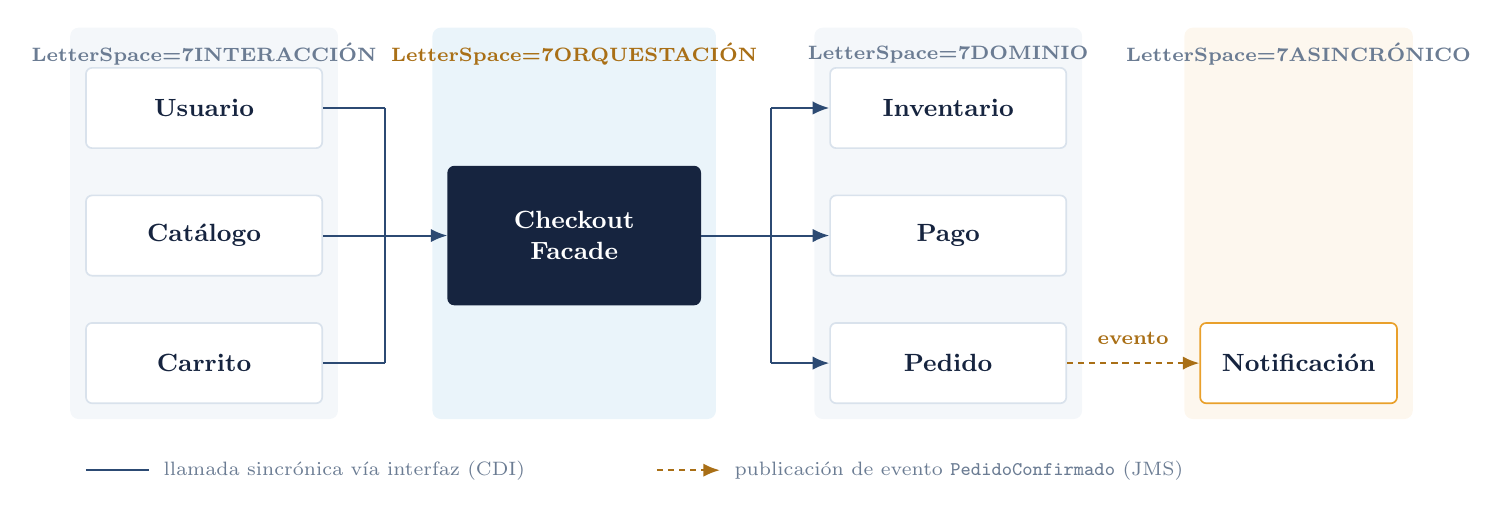
\begin{tikzpicture}[x=1cm,y=1cm]
  \def\ca{1.85}\def\cb{6.55}\def\cc{11.3}\def\cd{15.75}
  \def\ra{0}\def\rb{-1.62}\def\rc{-3.24}

  % ------- fondos de grupo
  \begin{scope}[on background layer]
    \fill[surface,rounded corners=3pt] (0.15,1.02) rectangle (3.55,-3.95);
    \fill[pale,rounded corners=3pt]    (4.75,1.02) rectangle (8.35,-3.95);
    \fill[surface,rounded corners=3pt] (9.6,1.02)  rectangle (13.0,-3.95);
    \fill[amber!8,rounded corners=3pt] (14.3,1.02) rectangle (17.2,-3.95);
  \end{scope}

  % ------- etiquetas de grupo
  \node[lbl,font=\scriptsize\bfseries,text=muted]   at (\ca,0.68) {\track{7}{INTERACCIÓN}};
  \node[lbl,font=\scriptsize\bfseries,text=amberdk] at (\cb,0.68) {\track{7}{ORQUESTACIÓN}};
  \node[lbl,font=\scriptsize\bfseries,text=muted]   at (\cc,0.68) {\track{7}{DOMINIO}};
  \node[lbl,font=\scriptsize\bfseries,text=muted]   at (\cd,0.68) {\track{7}{ASINCRÓNICO}};

  % ------- nodos
  \tikzset{comp/.style={cbox,minimum width=3.0cm,minimum height=1.02cm}}
  \node[comp] (usu) at (\ca,\ra) {Usuario};
  \node[comp] (cat) at (\ca,\rb) {Catálogo};
  \node[comp] (car) at (\ca,\rc) {Carrito};

  \node[cbox,fill=navy,draw=navy,text=white,minimum width=3.2cm,minimum height=1.75cm]
       (chk) at (\cb,\rb) {Checkout\\Facade};

  \node[comp] (inv) at (\cc,\ra) {Inventario};
  \node[comp] (pag) at (\cc,\rb) {Pago};
  \node[comp] (ped) at (\cc,\rc) {Pedido};

  \node[cbox,fill=white,draw=amber,minimum width=2.5cm,minimum height=1.02cm]
       (not) at (\cd,\rc) {Notificación};

  % ------- bus izquierdo
  \draw[line width=0.75pt,draw=steel] (usu.east) -- (4.15,\ra);
  \draw[line width=0.75pt,draw=steel] (cat.east) -- (4.15,\rb);
  \draw[line width=0.75pt,draw=steel] (car.east) -- (4.15,\rc);
  \draw[line width=0.75pt,draw=steel] (4.15,\ra) -- (4.15,\rc);
  \draw[call] (4.15,\rb) -- (chk.west);

  % ------- bus derecho
  \draw[line width=0.75pt,draw=steel] (chk.east) -- (9.05,\rb);
  \draw[line width=0.75pt,draw=steel] (9.05,\ra) -- (9.05,\rc);
  \draw[call] (9.05,\ra) -- (inv.west);
  \draw[call] (9.05,\rb) -- (pag.west);
  \draw[call] (9.05,\rc) -- (ped.west);

  % ------- evento asincrónico
  \draw[evt] (ped.east) -- (not.west);
  \node[lbl,text=amberdk,font=\scriptsize\bfseries] at (13.65,\rc+0.32) {evento};

  % ------- referencias
  \draw[line width=0.75pt,draw=steel] (0.35,-4.6) -- (1.15,-4.6);
  \node[lbl,anchor=west] at (1.28,-4.6) {llamada sincrónica vía interfaz (CDI)};
  \draw[evt] (7.6,-4.6) -- (8.4,-4.6);
  \node[lbl,anchor=west] at (8.53,-4.6) {publicación de evento \texttt{PedidoConfirmado} (JMS)};
\end{tikzpicture}
\end{center}

\vspace{2mm}
\begin{softbox}
\textbf{Criterio de diseño.} \texttt{CheckoutFacade} actúa como único orquestador: coordina carrito, inventario, pago y pedido sin duplicar sus reglas internas. Ningún componente de dominio conoce a otro directamente, y Notificación queda desacoplada mediante mensajería: si el envío del aviso falla, la compra ya está confirmada igual.
\end{softbox}

\newpage

% =============================================================================
% 03 · CAPAS  (diagrama principal)
% =============================================================================
\sectiontitle{03 · ARQUITECTURA DE CAPAS}{Presentación\arr Negocio\arr Datos}

Las tres capas son separaciones \textbf{lógicas} y se despliegan juntas en un único WAR. Cada capa se comunica solamente con la inmediatamente inferior y siempre a través de un contrato: nunca contra una implementación concreta.

\vspace{2mm}
\begin{center}
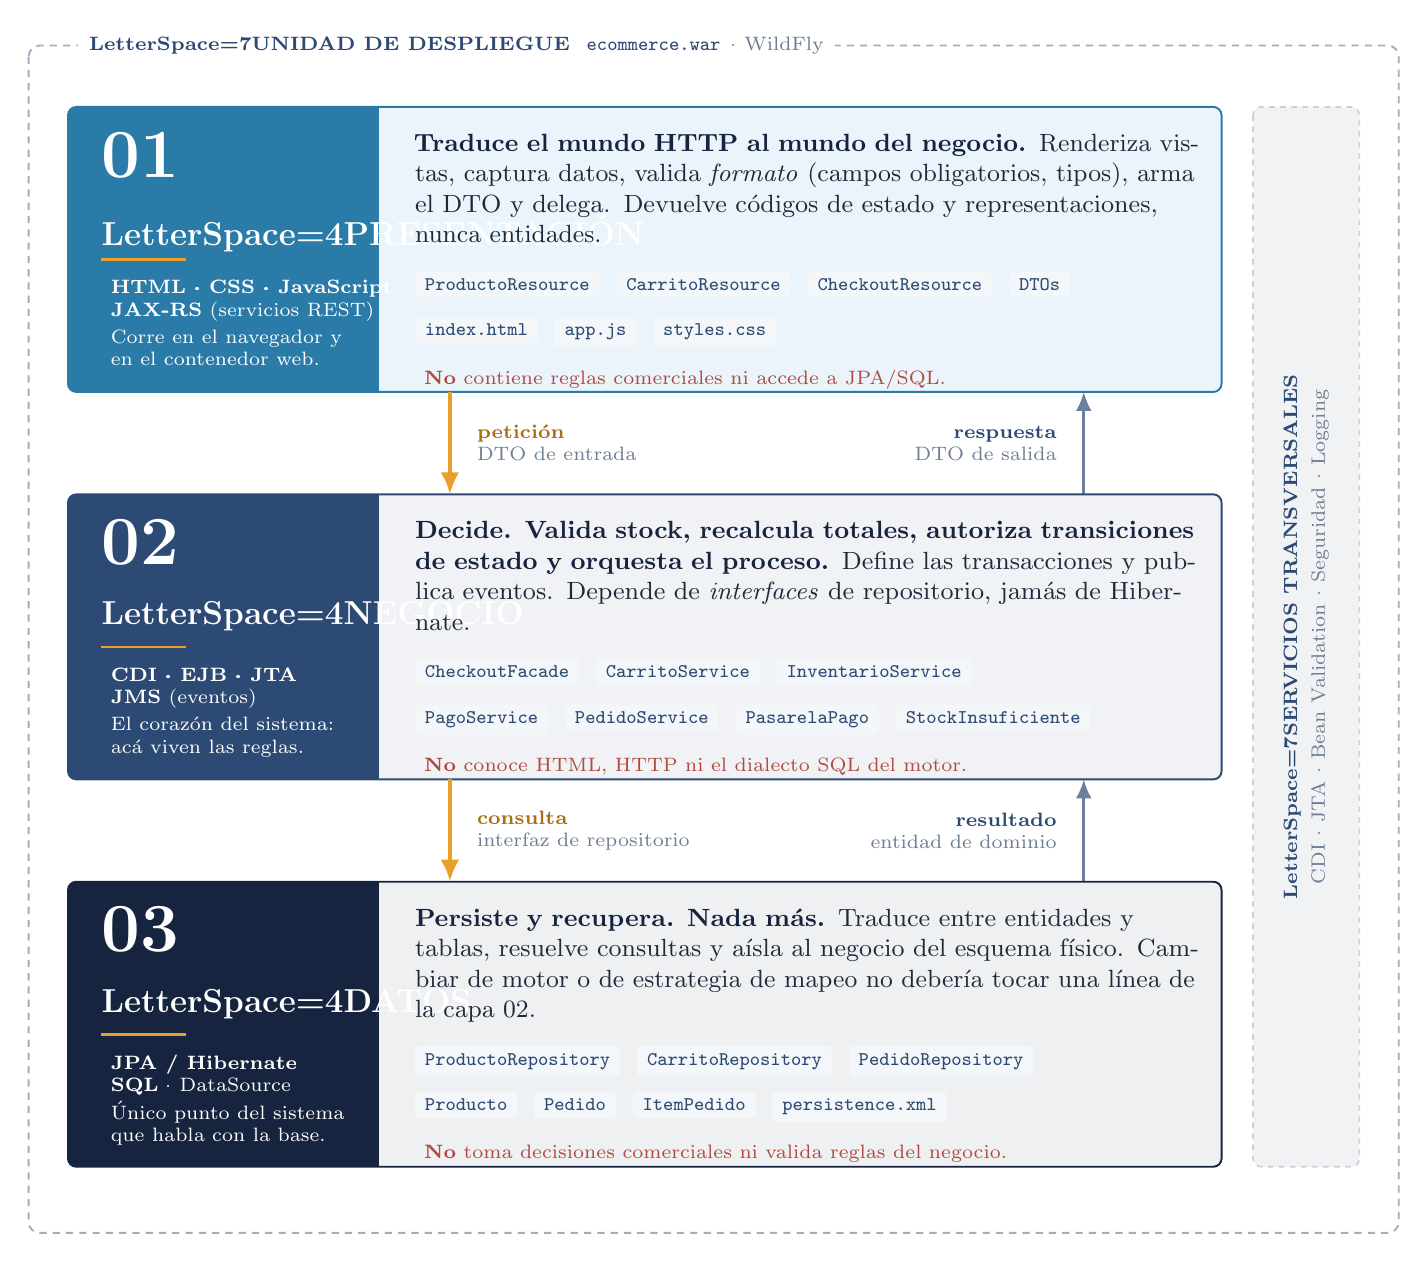
\begin{tikzpicture}[x=1cm,y=1cm,font=\small]
  % ---------------- geometría
  \def\XA{0.5}\def\XH{4.45}\def\XB{15.15}
  \def\XRA{15.55}\def\XRB{16.9}
  \def\BH{3.62}
  \def\YA{0}\def\YB{-4.92}\def\YC{-9.84}
  \def\XDN{5.35}\def\XUP{13.4}

  % ---------------- límite de despliegue
  \draw[draw=steel!45,dash pattern=on 2.6pt off 2.2pt,line width=0.7pt,rounded corners=4pt]
        (0,0.78) rectangle (17.4,-14.3);
  \node[anchor=west,fill=white,inner xsep=4pt,font=\scriptsize,text=steel]
        at (0.62,0.78) {\bfseries\track{7}{UNIDAD DE DESPLIEGUE}\ \ \normalfont\ttfamily
                        ecommerce.war \normalfont\color{muted}· WildFly};

  % ---------------- rail de servicios transversales
  \fill[navy!6,rounded corners=3pt] (\XRA,\YA) rectangle (\XRB,\YC-\BH);
  \draw[draw=navy!22,dash pattern=on 2pt off 2pt,line width=0.6pt,rounded corners=3pt]
        (\XRA,\YA) rectangle (\XRB,\YC-\BH);
  \node[rotate=90,font=\scriptsize\bfseries,text=steel,align=center]
        at ({(\XRA+\XRB)/2},{(\YA+\YC-\BH)/2})
        {\track{7}{SERVICIOS TRANSVERSALES}\\[2pt]
         \normalfont\scriptsize\color{muted} CDI · JTA · Bean Validation · Seguridad · Logging};

  % =========================================================== BANDA 01
  \begin{scope}
    \clip[rounded corners=3pt] (\XA,\YA) rectangle (\XB,\YA-\BH);
    \fill[white] (\XA,\YA) rectangle (\XB,\YA-\BH);
    \fill[brand] (\XA,\YA) rectangle (\XH,\YA-\BH);
    \fill[pale]  (\XH,\YA) rectangle (\XB,\YA-\BH);
  \end{scope}
  \draw[rounded corners=3pt,draw=brand,line width=0.7pt] (\XA,\YA) rectangle (\XB,\YA-\BH);
  \node[anchor=north west,text=white,inner sep=0]
        at (\XA+0.42,\YA-0.32) {\displayfont\fontsize{26}{26}\selectfont\bfseries 01};
  \node[anchor=north west,text=white,inner sep=0]
        at (\XA+0.42,\YA-1.36) {\displayfont\fontsize{12.5}{14}\selectfont\bfseries \track{4}{PRESENTACIÓN}};
  \draw[amber,line width=1pt] (\XA+0.42,\YA-1.94) -- (\XA+1.5,\YA-1.94);
  \node[anchor=north west,text=white,align=left,font=\scriptsize]
        at (\XA+0.42,\YA-2.08) {\textbf{HTML · CSS · JavaScript}\\ \textbf{JAX-RS} (servicios REST)\\[2pt]
                                \color{white!72}Corre en el navegador y\\ \color{white!72}en el contenedor web.};
  \node[anchor=north west,text width=9.9cm,align=left,font=\small,text=ink,inner sep=0]
        at (\XH+0.45,\YA-0.34)
        {\textbf{\color{navy}Traduce el mundo HTTP al mundo del negocio.} Renderiza vistas, captura datos, valida \emph{formato} (campos obligatorios, tipos), arma el DTO y delega. Devuelve códigos de estado y representaciones, nunca entidades.};
  \node[chip] (p1) at (\XH+0.45,\YA-2.08) {ProductoResource};
  \node[chip] (p2) at ([xshift=2mm]p1.north east) {CarritoResource};
  \node[chip] (p3) at ([xshift=2mm]p2.north east) {CheckoutResource};
  \node[chip] (p4) at ([xshift=2mm]p3.north east) {DTOs};
  \node[chip] (p5) at (\XH+0.45,\YA-2.66) {index.html};
  \node[chip] (p6) at ([xshift=2mm]p5.north east) {app.js};
  \node[chip] (p7) at ([xshift=2mm]p6.north east) {styles.css};
  \node[anchor=north west,font=\scriptsize,text=no]
        at (\XH+0.45,\YA-3.22) {\textbf{No} contiene reglas comerciales ni accede a JPA/SQL.};

  % ---------------- conectores 01 → 02
  \draw[-{Latex[length=2.8mm,width=2.4mm]},line width=1.5pt,draw=amber]
        (\XDN,\YA-\BH) -- (\XDN,\YB);
  \node[anchor=west,font=\scriptsize\bfseries,text=amberdk,align=left]
        at (\XDN+0.22,{(\YA-\BH+\YB)/2}) {petición\\\normalfont\color{muted}DTO de entrada};
  \draw[-{Latex[length=2.4mm,width=2.0mm]},line width=1pt,draw=steel!70]
        (\XUP,\YB) -- (\XUP,\YA-\BH);
  \node[anchor=east,font=\scriptsize\bfseries,text=steel,align=right]
        at (\XUP-0.22,{(\YA-\BH+\YB)/2}) {respuesta\\\normalfont\color{muted}DTO de salida};

  % =========================================================== BANDA 02
  \begin{scope}
    \clip[rounded corners=3pt] (\XA,\YB) rectangle (\XB,\YB-\BH);
    \fill[white] (\XA,\YB) rectangle (\XB,\YB-\BH);
    \fill[steel] (\XA,\YB) rectangle (\XH,\YB-\BH);
    \fill[steel!7](\XH,\YB) rectangle (\XB,\YB-\BH);
  \end{scope}
  \draw[rounded corners=3pt,draw=steel,line width=0.7pt] (\XA,\YB) rectangle (\XB,\YB-\BH);
  \node[anchor=north west,text=white,inner sep=0]
        at (\XA+0.42,\YB-0.32) {\displayfont\fontsize{26}{26}\selectfont\bfseries 02};
  \node[anchor=north west,text=white,inner sep=0]
        at (\XA+0.42,\YB-1.36) {\displayfont\fontsize{12.5}{14}\selectfont\bfseries \track{4}{NEGOCIO}};
  \draw[amber,line width=1pt] (\XA+0.42,\YB-1.94) -- (\XA+1.5,\YB-1.94);
  \node[anchor=north west,text=white,align=left,font=\scriptsize]
        at (\XA+0.42,\YB-2.08) {\textbf{CDI · EJB · JTA}\\ \textbf{JMS} (eventos)\\[2pt]
                                \color{white!72}El corazón del sistema:\\ \color{white!72}acá viven las reglas.};
  \node[anchor=north west,text width=9.9cm,align=left,font=\small,text=ink,inner sep=0]
        at (\XH+0.45,\YB-0.34)
        {\textbf{\color{navy}Decide. Valida stock, recalcula totales, autoriza transiciones de estado y orquesta el proceso.} Define las transacciones y publica eventos. Depende de \emph{interfaces} de repositorio, jamás de Hibernate.};
  \node[chip] (n1) at (\XH+0.45,\YB-2.08) {CheckoutFacade};
  \node[chip] (n2) at ([xshift=2mm]n1.north east) {CarritoService};
  \node[chip] (n3) at ([xshift=2mm]n2.north east) {InventarioService};
  \node[chip] (n4) at (\XH+0.45,\YB-2.66) {PagoService};
  \node[chip] (n5) at ([xshift=2mm]n4.north east) {PedidoService};
  \node[chip] (n6) at ([xshift=2mm]n5.north east) {PasarelaPago};
  \node[chip] (n7) at ([xshift=2mm]n6.north east) {StockInsuficiente};
  \node[anchor=north west,font=\scriptsize,text=no]
        at (\XH+0.45,\YB-3.22) {\textbf{No} conoce HTML, HTTP ni el dialecto SQL del motor.};

  % ---------------- conectores 02 → 03
  \draw[-{Latex[length=2.8mm,width=2.4mm]},line width=1.5pt,draw=amber]
        (\XDN,\YB-\BH) -- (\XDN,\YC);
  \node[anchor=west,font=\scriptsize\bfseries,text=amberdk,align=left]
        at (\XDN+0.22,{(\YB-\BH+\YC)/2}) {consulta\\\normalfont\color{muted}interfaz de repositorio};
  \draw[-{Latex[length=2.4mm,width=2.0mm]},line width=1pt,draw=steel!70]
        (\XUP,\YC) -- (\XUP,\YB-\BH);
  \node[anchor=east,font=\scriptsize\bfseries,text=steel,align=right]
        at (\XUP-0.22,{(\YB-\BH+\YC)/2}) {resultado\\\normalfont\color{muted}entidad de dominio};

  % =========================================================== BANDA 03
  \begin{scope}
    \clip[rounded corners=3pt] (\XA,\YC) rectangle (\XB,\YC-\BH);
    \fill[white] (\XA,\YC) rectangle (\XB,\YC-\BH);
    \fill[navy]  (\XA,\YC) rectangle (\XH,\YC-\BH);
    \fill[navy!7](\XH,\YC) rectangle (\XB,\YC-\BH);
  \end{scope}
  \draw[rounded corners=3pt,draw=navy,line width=0.7pt] (\XA,\YC) rectangle (\XB,\YC-\BH);
  \node[anchor=north west,text=white,inner sep=0]
        at (\XA+0.42,\YC-0.32) {\displayfont\fontsize{26}{26}\selectfont\bfseries 03};
  \node[anchor=north west,text=white,inner sep=0]
        at (\XA+0.42,\YC-1.36) {\displayfont\fontsize{12.5}{14}\selectfont\bfseries \track{4}{DATOS}};
  \draw[amber,line width=1pt] (\XA+0.42,\YC-1.94) -- (\XA+1.5,\YC-1.94);
  \node[anchor=north west,text=white,align=left,font=\scriptsize]
        at (\XA+0.42,\YC-2.08) {\textbf{JPA / Hibernate}\\ \textbf{SQL} · DataSource\\[2pt]
                                \color{white!72}Único punto del sistema\\ \color{white!72}que habla con la base.};
  \node[anchor=north west,text width=9.9cm,align=left,font=\small,text=ink,inner sep=0]
        at (\XH+0.45,\YC-0.34)
        {\textbf{\color{navy}Persiste y recupera. Nada más.} Traduce entre entidades y tablas, resuelve consultas y aísla al negocio del esquema físico. Cambiar de motor o de estrategia de mapeo no debería tocar una línea de la capa 02.};
  \node[chip] (d1) at (\XH+0.45,\YC-2.08) {ProductoRepository};
  \node[chip] (d2) at ([xshift=2mm]d1.north east) {CarritoRepository};
  \node[chip] (d3) at ([xshift=2mm]d2.north east) {PedidoRepository};
  \node[chip] (d4) at (\XH+0.45,\YC-2.66) {Producto};
  \node[chip] (d5) at ([xshift=2mm]d4.north east) {Pedido};
  \node[chip] (d6) at ([xshift=2mm]d5.north east) {ItemPedido};
  \node[chip] (d7) at ([xshift=2mm]d6.north east) {persistence.xml};
  \node[anchor=north west,font=\scriptsize,text=no]
        at (\XH+0.45,\YC-3.22) {\textbf{No} toma decisiones comerciales ni valida reglas del negocio.};
\end{tikzpicture}
\end{center}

\vspace{1mm}
\begin{minipage}[t]{0.485\linewidth}
\begin{listbox}[Permitido]{ok}
{\footnotesize
\begin{itemize}
  \item Controller\arrs Service\arrs Repository.
  \item Inyectar dependencias contra interfaces.
  \item Declarar la transacción en la capa 02.
  \item Devolver DTOs hacia afuera.
\end{itemize}}
\end{listbox}
\end{minipage}\hfill
\begin{minipage}[t]{0.485\linewidth}
\begin{listbox}[No permitido]{no}
{\footnotesize
\begin{itemize}
  \item Vista o controller consultando JPA/SQL.
  \item Repository decidiendo reglas comerciales.
  \item Service importando clases HTTP.
  \item Saltar una capa para ``resolver rápido''.
\end{itemize}}
\end{listbox}
\end{minipage}

\newpage

% =============================================================================
% 04 · CASO DE USO (diagrama de secuencia)
% =============================================================================
\sectiontitle{04 · RECORRIDO ENTRE CAPAS}{Caso de uso: confirmar una compra}

Una petición completa, paso a paso: llamadas sincrónicas en línea llena, retornos punteados, y el evento asincrónico saliendo del marco transaccional.

\vspace{-1mm}
\begin{center}
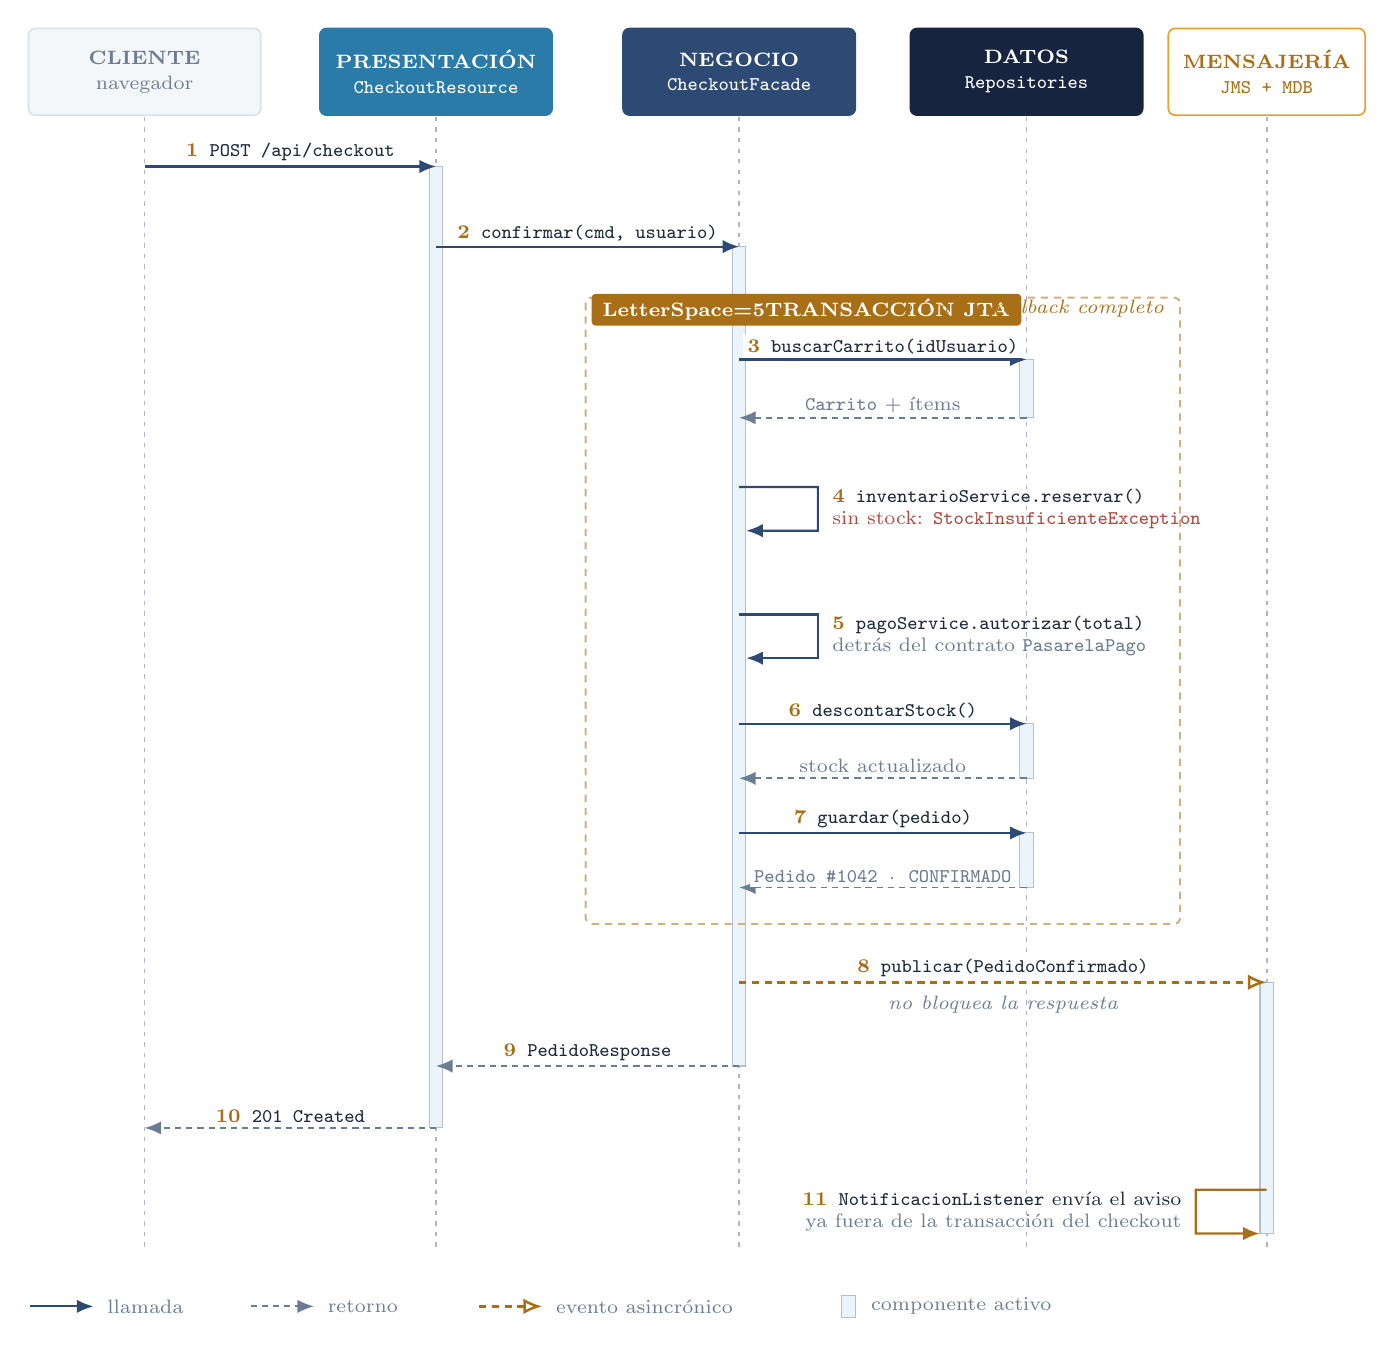
\begin{tikzpicture}[x=1cm,y=0.925cm,font=\small]
  \def\LA{1.75}\def\LB{5.45}\def\LC{9.3}\def\LD{12.95}\def\LE{16.0}

  \tikzset{
    lane/.style={draw=rule,line width=0.6pt,rounded corners=2.4pt,fill=white,
                 minimum width=2.95cm,minimum height=1.1cm,align=center,
                 font=\scriptsize\bfseries,text=navy,inner sep=2pt},
    life/.style={draw=steel!40,line width=0.6pt,dash pattern=on 1.6pt off 2.2pt},
    act/.style={draw=steel!35,line width=0.4pt,fill=pale},
    msg/.style={-{Latex[length=2.1mm,width=1.7mm]},line width=0.8pt,draw=steel},
    ret/.style={-{Latex[length=2.1mm,width=1.7mm]},line width=0.65pt,draw=muted,
                dash pattern=on 2.2pt off 1.8pt},
    async/.style={-{Latex[length=2.4mm,width=2.0mm,open]},line width=0.9pt,draw=amberdk,
                dash pattern=on 2.6pt off 2pt},
    m/.style={font=\scriptsize,text=ink,inner sep=1.6pt,fill=white},
  }
  \newcommand{\nm}[1]{{\bfseries\color{amberdk}#1}\,}

  % --------- encabezados
  \node[lane,fill=surface,text=muted]         (ha) at (\LA,0) {CLIENTE\\[1pt]\normalfont\scriptsize navegador};
  \node[lane,fill=brand,draw=brand,text=white](hb) at (\LB,0) {PRESENTACIÓN\\[1pt]\normalfont\scriptsize\ttfamily CheckoutResource};
  \node[lane,fill=steel,draw=steel,text=white](hc) at (\LC,0) {NEGOCIO\\[1pt]\normalfont\scriptsize\ttfamily CheckoutFacade};
  \node[lane,fill=navy,draw=navy,text=white]  (hd) at (\LD,0) {DATOS\\[1pt]\normalfont\scriptsize\ttfamily Repositories};
  \node[lane,fill=white,draw=amber,text=amberdk,minimum width=2.5cm]
                                              (he) at (\LE,0) {MENSAJERÍA\\[1pt]\normalfont\scriptsize\ttfamily JMS + MDB};

  % --------- líneas de vida
  \foreach \x in {\LA,\LB,\LC,\LD,\LE} { \draw[life] (\x,-0.62) -- (\x,-16.2); }

  % --------- barras de activación
  \fill[act] (\LB-0.085,-1.30) rectangle (\LB+0.085,-14.50);
  \fill[act] (\LC-0.085,-2.40) rectangle (\LC+0.085,-13.65);
  \fill[act] (\LD-0.085,-3.95) rectangle (\LD+0.085,-4.75);
  \fill[act] (\LD-0.085,-8.95) rectangle (\LD+0.085,-9.70);
  \fill[act] (\LD-0.085,-10.45) rectangle (\LD+0.085,-11.20);
  \fill[act] (\LE-0.085,-12.50) rectangle (\LE+0.085,-15.95);

  % --------- marco transaccional (fragmento UML)
  \draw[draw=amberdk!55,line width=0.7pt,dash pattern=on 2.6pt off 2.2pt,rounded corners=2pt]
        (7.35,-3.10) rectangle (14.9,-11.70);
  \node[anchor=north west,fill=amberdk,text=white,font=\scriptsize\bfseries,
        inner xsep=4pt,inner ysep=1.8pt,rounded corners=1.4pt] at (7.42,-3.04)
        {\track{5}{TRANSACCIÓN JTA}};
  \node[anchor=north east,font=\scriptsize\itshape,text=amberdk] at (14.82,-3.0)
        {commit o rollback completo};

  % --------- mensajes
  \draw[msg] (\LA,-1.30) -- (\LB,-1.30)
        node[m,midway,above]{\nm{1} \texttt{POST /api/checkout}};
  \draw[msg] (\LB,-2.40) -- (\LC,-2.40)
        node[m,midway,above]{\nm{2} \texttt{confirmar(cmd, usuario)}};
  \draw[msg] (\LC,-3.95) -- (\LD,-3.95)
        node[m,midway,above]{\nm{3} \texttt{buscarCarrito(idUsuario)}};
  \draw[ret] (\LD,-4.75) -- (\LC,-4.75)
        node[m,midway,above]{\color{muted}\texttt{Carrito} + ítems};

  % self-call: reservar stock
  \draw[msg] (\LC,-5.70) -- ++(1.0,0) -- ++(0,-0.6) -- (\LC+0.09,-6.30);
  \node[m,anchor=west,align=left,fill=none] at (\LC+1.12,-6.00)
        {\nm{4} \texttt{inventarioService.reservar()}\\
         \color{no}sin stock: \texttt{StockInsuficienteException}};

  % self-call: pago
  \draw[msg] (\LC,-7.45) -- ++(1.0,0) -- ++(0,-0.6) -- (\LC+0.09,-8.05);
  \node[m,anchor=west,align=left,fill=none] at (\LC+1.12,-7.75)
        {\nm{5} \texttt{pagoService.autorizar(total)}\\
         \color{muted}detrás del contrato \texttt{PasarelaPago}};

  \draw[msg] (\LC,-8.95) -- (\LD,-8.95)
        node[m,midway,above]{\nm{6} \texttt{descontarStock()}};
  \draw[ret] (\LD,-9.70) -- (\LC,-9.70)
        node[m,midway,above]{\color{muted}stock actualizado};

  \draw[msg] (\LC,-10.45) -- (\LD,-10.45)
        node[m,midway,above]{\nm{7} \texttt{guardar(pedido)}};
  \draw[ret] (\LD,-11.20) -- (\LC,-11.20)
        node[m,midway,above]{\color{muted}\texttt{Pedido \#1042 · CONFIRMADO}};

  \draw[async] (\LC,-12.50) -- (\LE,-12.50)
        node[m,midway,above]{\nm{8} \texttt{publicar(PedidoConfirmado)}};
  \node[m,anchor=north,text=muted,font=\scriptsize\itshape,fill=none]
        at ({(\LC+\LE)/2},-12.62) {no bloquea la respuesta};

  \draw[ret] (\LC,-13.65) -- (\LB,-13.65)
        node[m,midway,above]{\nm{9} \texttt{PedidoResponse}};
  \draw[ret] (\LB,-14.50) -- (\LA,-14.50)
        node[m,midway,above]{\nm{10} \texttt{201 Created}};

  \draw[msg,draw=amberdk] (\LE,-15.35) -- ++(-0.9,0) -- ++(0,-0.6) -- (\LE-0.09,-15.95);
  \node[m,anchor=east,align=right,fill=none] at (\LE-1.02,-15.65)
        {\nm{11} \texttt{NotificacionListener} envía el aviso\\
         \color{muted}ya fuera de la transacción del checkout};

  % --------- referencias
  \draw[msg]   (0.30,-16.95) -- (1.10,-16.95);
  \node[lbl,anchor=west] at (1.22,-16.95) {llamada};
  \draw[ret]   (3.10,-16.95) -- (3.90,-16.95);
  \node[lbl,anchor=west] at (4.02,-16.95) {retorno};
  \draw[async] (6.00,-16.95) -- (6.80,-16.95);
  \node[lbl,anchor=west] at (6.92,-16.95) {evento asincrónico};
  \fill[act] (10.60,-17.10) rectangle (10.78,-16.80);
  \node[lbl,anchor=west] at (10.92,-16.95) {componente activo};
\end{tikzpicture}
\end{center}

\vspace{-2mm}
\begin{callout}
\textbf{Reglas demostrables en la defensa:} el total \emph{siempre} se recalcula en el servidor —nunca se confía en el precio que manda el cliente—; no hay confirmación sin stock reservado y pago aprobado; cualquier fallo dentro del marco JTA revierte la transacción completa y responde \texttt{409 Conflict}; y la notificación, al ser asincrónica, no puede demorar ni romper el checkout.
\end{callout}

\newpage

% =============================================================================
% 05 · PATRONES
% =============================================================================
\sectiontitle{05 · DISEÑO Y CALIDAD}{Patrones aplicados con una razón concreta}

Ningún patrón entra ``porque sí''. Cada uno resuelve un problema puntual de este proyecto.

\vspace{1mm}
{\footnotesize
\rowcolors{2}{surface}{white}
\begin{tabularx}{\linewidth}{N{2.55cm} M{4.5cm} X}
\toprule
\thd{PATRÓN / ROL} & \thd{DÓNDE} & \thd{POR QUÉ} \\
\midrule
Controller         & ProductoResource, CheckoutResource   & Traduce HTTP y delega; evita controllers ``gordos''. \\
Service Layer      & CarritoService, PedidoService        & Centraliza las reglas y los casos de uso. \\
Repository / DAO   & ProductoRepository, PedidoRepository & Encapsula JPA y permite probar el negocio aislado. \\
DTO                & AgregarItemRequest, PedidoResponse   & Separa el contrato web de las entidades persistentes. \\
Facade             & CheckoutFacade                       & Simplifica un proceso que coordina varios componentes. \\
Adapter            & PasarelaPagoSimuladaAdapter          & Desacopla el proveedor de pagos del checkout. \\
Factory            & NotificadorFactory                   & Selecciona el canal sin acoplar al consumidor. \\
Observer / Pub-Sub & evento PedidoConfirmado (JMS)        & Desacopla la compra de las tareas posteriores. \\
\bottomrule
\end{tabularx}}
\rowcolors{1}{}{}

\vspace{3.5mm}
\blocktitle{Estructura de paquetes propuesta}
\vspace{1.5mm}
\begin{whitebox}
{\scriptsize
\setlength{\arrayrulewidth}{0pt}
\renewcommand{\arraystretch}{1.14}
\begin{tabular}{@{}>{\ttfamily\color{steel}}l@{\hspace{6mm}}>{\color{muted}}l@{}}
\multicolumn{2}{@{}l}{\ttfamily\color{navy}\bfseries src/main/java/ar/edu/desarrolloappii/ecommerce/} \\
\hspace*{3mm}config/                                              & arranque, datasource, configuración de JAX-RS \\
\hspace*{3mm}shared/\{dto, exception\}/                           & contratos y errores comunes a todos \\
\hspace*{3mm}usuario/\{controller, service, repository, domain\}/ & \\
\hspace*{3mm}catalogo/\{controller, service, repository, domain\}/& \\
\hspace*{3mm}inventario/\{service, repository, domain\}/          & sin controller: lo usa el checkout \\
\hspace*{3mm}carrito/\{controller, service, repository, domain\}/ & \\
\hspace*{3mm}pedido/\{controller, service, repository, domain\}/  & \\
\hspace*{3mm}pago/\{service, adapter, domain\}/                   & el \textit{adapter} aísla la pasarela \\
\hspace*{3mm}checkout/\{controller, facade, dto\}/                & el orquestador del caso de uso \\
\hspace*{3mm}notificacion/\{listener, service, factory\}/         & consumidor JMS \\
\end{tabular}}
\end{whitebox}

\begin{softbox}
\textbf{Decisión estructural:} organizamos \emph{primero por componente y después por capa}. Así el árbol de paquetes grita qué hace el sistema (catálogo, carrito, pedido) y no con qué framework está hecho. Las capas siguen siendo explícitas dentro de cada componente —\texttt{controller}\arrs\texttt{service}\arrs\texttt{repository}— pero evitamos las tres carpetas globales gigantes que terminan mezclando todo.
\end{softbox}

\vspace{1mm}
\blocktitle{Principios de revisión}
{\small
\begin{itemize}
  \item \textbf{Alta cohesión:} cada clase y cada componente tiene una responsabilidad precisa.
  \item \textbf{Bajo acoplamiento:} la colaboración pasa siempre por interfaces e inyección CDI.
  \item \textbf{Configuración externa:} datasource, URLs y credenciales nunca hardcodeados.
  \item \textbf{Testabilidad:} services probables sin levantar la interfaz web; repositories con pruebas de integración.
  \item \textbf{Consistencia:} diagramas, nombres de clases, código y defensa oral describen la misma arquitectura.
\end{itemize}}

\newpage

% =============================================================================
% 06 · STACK Y ENTREGABLE
% =============================================================================
\sectiontitle{06 · TECNOLOGÍA Y ENTREGABLE}{Stack elegido y verificación de la consigna}

\vspace{-1mm}
{\footnotesize
\rowcolors{2}{surface}{white}
\begin{tabularx}{\linewidth}{N{2.75cm} L{4.6cm} X}
\toprule
\thd{ÁREA} & \thd{TECNOLOGÍA} & \thd{POR QUÉ ESTA Y NO OTRA} \\
\midrule
Entorno      & \color{steel}Visual Studio Code + JDK 17+ & Reemplaza a Eclipse sin alterar Maven ni Jakarta EE. \\
Construcción & \color{steel}Apache Maven                 & Dependencias reproducibles y generación del WAR. \\
Presentación & \color{steel}HTML/CSS/JS + JAX-RS         & UI simple y API clara; adaptable a JSP/JSF si se pide. \\
Negocio      & \color{steel}CDI + EJB + JTA              & Inyección, ciclo de vida y transacciones del contenedor. \\
Datos        & \color{steel}JPA / Hibernate + SQL        & Persistencia desacoplada detrás de repositories. \\
Mensajería   & \color{steel}JMS + Message-Driven Bean    & Integración asincrónica para notificaciones. \\
Servidor     & \color{steel}WildFly                      & Servidor de referencia indicado en las clases. \\
Empaquetado  & \color{steel}WAR                          & Una sola unidad desplegable, acorde al tamaño del TP. \\
\bottomrule
\end{tabularx}}
\rowcolors{1}{}{}

\vspace{4mm}
\blocktitle{Cumplimiento de la consigna del taller}
\vspace{1.5mm}
\begin{whitebox}
{\small
\renewcommand{\arraystretch}{1.35}
\begin{tabularx}{\linewidth}{@{}m{6mm} X @{\hspace{4mm}} >{\footnotesize\raggedright\arraybackslash\color{muted}}m{3.0cm}@{}}
\tick & Se retomaron y ampliaron los componentes identificados en el TP inicial. & sección 02 \\
\tick & Se agruparon según su responsabilidad: presentación, negocio o datos.   & sección 03 \\
\tick & Se eligió una tecnología concreta para cada capa.                       & secciones 03 y 06 \\
\tick & Se dibujó el diagrama de arquitectura en capas.                         & sección 03 \\
\tick & Se describió la responsabilidad puntual de cada capa.                   & sección 03 \\
\tick & Se documentó ``confirmar compra'' atravesando las tres capas.           & sección 04 \\
\tick & Se justificaron contratos, dependencias y patrones de diseño.           & secciones 02 y 05 \\
\end{tabularx}}
\end{whitebox}

\vspace{2mm}
\blocktitle{Próximos pasos de implementación}
{\small
\begin{enumerate}[itemsep=1.5pt]
  \item Cerrar alcance e integrantes; crear el proyecto Maven y desplegar un endpoint mínimo en WildFly.
  \item Implementar catálogo, carrito, persistencia y checkout respetando estrictamente las tres capas.
  \item Incorporar JMS, servicios web y pruebas; mantener documentación y código sincronizados clase a clase.
\end{enumerate}}

\vspace{2mm}
\begin{callout}
\textbf{Conclusión.} El diseño cumple la primera parte solicitada: identifica los componentes, los organiza por responsabilidad, elige el stack de cada capa, representa la arquitectura y demuestra un caso de uso completo de punta a punta. Y lo más importante: puede crecer clase a clase sin tocar su estructura central.
\end{callout}

\vspace{1mm}
{\footnotesize\color{muted}Documento elaborado a partir de las presentaciones de las clases 1, 2 y 3 de Desarrollo de Aplicaciones II. Fecha y cronograma de entrega sujetos a confirmación del docente.}

\end{document}
